\documentclass{beamer}
\mode<presentation>{
  \usetheme{Boadilla}
  \usefonttheme[onlylarge]{structurebold}
  \usefonttheme[stillsansseriflarge]{serif}
  \setbeamerfont*{frametitle}{size=\normalsize,series=\bfseries}
  % \setbeamertemplate{navigation symbols}{}
  \setbeamercovered{transparent}
}
\usepackage[english]{babel}
\usepackage[latin1]{inputenc}
\usepackage{times}
\usepackage[T1]{fontenc}
\usepackage{amsmath}
\usepackage{amssymb}
\usepackage{esint}
\usepackage{hyperref}
\usepackage{tikz}
\usepackage{xkeyval}
\usepackage{xargs}
\usepackage{xcolor}
\usepackage{verbatim}
\usepackage{listings}
\usepackage{multimedia}
\usepackage{bm}
\usepackage{siunitx}
\usetikzlibrary{
  arrows,
  calc,
  decorations.pathmorphing,
  decorations.pathreplacing,
  decorations.markings,
  fadings,
  positioning,
  shapes,
  arrows.meta
}
\usepgfmodule{oo}

\pgfdeclareradialshading{glow2}{\pgfpoint{0cm}{0cm}}{
  color(0mm)=(white);
  color(2mm)=(white);
  color(8mm)=(black);
  color(10mm)=(black)
}
\pgfdeclareradialshading{glow}{\pgfpoint{0cm}{0cm}}{
  color(0mm)=(white);
  color(5mm)=(white);
  color(9mm)=(black);
  color(10mm)=(black)
}
\pgfdeclareverticalshading{north edge}{2cm}{
  % manual 1082-1083; later - shading is assumed to be 100bp diameter ??
  color(0cm)=(white);
  color(1.3cm)=(white);
  color(1.5cm)=(black)
}

\begin{tikzfadingfrompicture}[name=glow fading]
  \shade [shading=glow] (0,0) circle (1);
\end{tikzfadingfrompicture}

\begin{tikzfadingfrompicture}[name=glow2 fading]
  \shade [shading=glow2] (0,0) circle (1);
\end{tikzfadingfrompicture}

\begin{tikzfadingfrompicture}[name=north edge fading]
  \shade [shading=north edge] (-1,-1) rectangle (1, 1);
\end{tikzfadingfrompicture}

\mode<handout>{
  \usepackage{pgfpages}
  \pgfpagesuselayout{4 on 1}[a4paper,landscape,border shrink=5mm]
  \setbeamercolor{background canvas}{bg=black!10}
}

\newcommand\pgfmathsinandcos[3]{%
  \pgfmathsetmacro#1{sin(#3)}%
  \pgfmathsetmacro#2{cos(#3)}%
}
\newcommand\LongitudePlane[3][current plane]{%
  \pgfmathsinandcos\sinEl\cosEl{#2} % elevation
  \pgfmathsinandcos\sint\cost{#3} % azimuth
  \tikzset{#1/.estyle={cm={\cost,\sint*\sinEl,0,\cosEl,(0,0)}}}
}
\newcommand\LatitudePlane[3][current plane]{%
  \pgfmathsinandcos\sinEl\cosEl{#2} % elevation
  \pgfmathsinandcos\sint\cost{#3} % latitude
  \pgfmathsetmacro\yshift{\cosEl*\sint}
  \tikzset{#1/.estyle={cm={\cost,0,0,\cost*\sinEl,(0,\yshift)}}} %
}
\newcommand\DrawLongitudeCircle[2][1]{
  \LongitudePlane{\angEl}{#2}
  \tikzset{current plane/.prefix style={scale=#1}}
  % angle of "visibility"
  \pgfmathsetmacro\angVis{atan(sin(#2)*cos(\angEl)/sin(\angEl))} %
  \draw[current plane] (\angVis:1) arc (\angVis:\angVis+180:1);
  \draw[current plane,dashed] (\angVis-180:1) arc (\angVis-180:\angVis:1);
}
\newcommand\DrawLatitudeCircleArrow[2][1]{
  \LatitudePlane{\angEl}{#2}
  \tikzset{current plane/.prefix style={scale=#1}}
  \pgfmathsetmacro\sinVis{sin(#2)/cos(#2)*sin(\angEl)/cos(\angEl)}
  % angle of "visibility"
  \pgfmathsetmacro\angVis{asin(min(1,max(\sinVis,-1)))}
  \draw[current plane,decoration={markings, mark=at position 0.6 with {\arrow{<}}},postaction={decorate},line width=.6mm] (\angVis:1) arc (\angVis:-\angVis-180:1);
  \draw[current plane,dashed,line width=.6mm] (180-\angVis:1) arc (180-\angVis:\angVis:1);
}
\newcommand\DrawLatitudeCircle[2][1]{
  \LatitudePlane{\angEl}{#2}
  \tikzset{current plane/.prefix style={scale=#1}}
  \pgfmathsetmacro\sinVis{sin(#2)/cos(#2)*sin(\angEl)/cos(\angEl)}
  % angle of "visibility"
  \pgfmathsetmacro\angVis{asin(min(1,max(\sinVis,-1)))}
  \draw[current plane] (\angVis:1) arc (\angVis:-\angVis-180:1);
  \draw[current plane,dashed] (180-\angVis:1) arc (180-\angVis:\angVis:1);
}
\newcommand\coil[1]{
  {\rh * cos(\t * pi r)}, {\apart * (2 * #1 + \t) + \rv * sin(\t * pi r)}
}
\makeatletter
\define@key{DrawFromCenter}{style}[{->}]{
  \tikzset{DrawFromCenterPlane/.style={#1}}
}
\define@key{DrawFromCenter}{r}[1]{
  \def\@R{#1}
}
\define@key{DrawFromCenter}{center}[(0, 0)]{
  \def\@Center{#1}
}
\define@key{DrawFromCenter}{theta}[0]{
  \def\@Theta{#1}
}
\define@key{DrawFromCenter}{phi}[0]{
  \def\@Phi{#1}
}
\presetkeys{DrawFromCenter}{style, r, center, theta, phi}{}
\newcommand*\DrawFromCenter[1][]{
  \setkeys{DrawFromCenter}{#1}{
    \pgfmathsinandcos\sint\cost{\@Theta}
    \pgfmathsinandcos\sinp\cosp{\@Phi}
    \pgfmathsinandcos\sinA\cosA{\angEl}
    \pgfmathsetmacro\DX{\@R*\cost*\cosp}
    \pgfmathsetmacro\DY{\@R*(\cost*\sinp*\sinA+\sint*\cosA)}
    \draw[DrawFromCenterPlane] \@Center -- ++(\DX, \DY);
  }
}
\newcommand*\DrawFromCenterText[2][]{
  \setkeys{DrawFromCenter}{#1}{
    \pgfmathsinandcos\sint\cost{\@Theta}
    \pgfmathsinandcos\sinp\cosp{\@Phi}
    \pgfmathsinandcos\sinA\cosA{\angEl}
    \pgfmathsetmacro\DX{\@R*\cost*\cosp}
    \pgfmathsetmacro\DY{\@R*(\cost*\sinp*\sinA+\sint*\cosA)}
    \draw[DrawFromCenterPlane] \@Center -- ++(\DX, \DY) node {#2};
  }
}
\makeatother

% not mandatory, but I though it was better to set it blank
\setbeamertemplate{headline}{}
\def\beamer@entrycode{\vspace{-\headheight}}

\tikzstyle{snakearrow} = [decorate, decoration={pre length=0.2cm,
  post length=0.2cm, snake, amplitude=.4mm,
  segment length=2mm},thick, ->]

%% document-wide tikz options and styles

\tikzset{%
  % >=latex, % option for nice arrows
  inner sep=0pt,%
  outer sep=2pt,%
  mark coordinate/.style={inner sep=0pt,outer sep=0pt,minimum size=3pt,
    fill=black,circle}%
}
\tikzset{
  % Define standard arrow tip
  >=stealth',
  % Define style for boxes
  punkt/.style={
    rectangle,
    rounded corners,
    draw=black, very thick,
    text width=8em,
    minimum height=2.5em,
    text centered},
}

\tikzset{onslide/.code args={<#1>#2}{%
    \only<#1>{\pgfkeysalso{#2}}
    % \pgfkeysalso doesn't change the path
  }}
\tikzset{alt/.code args={<#1>#2#3}{%
    \alt<#1>{\pgfkeysalso{#2}}{\pgfkeysalso{#3}}
    % \pgfkeysalso doesn't change the path
  }}
\tikzset{temporal/.code args={<#1>#2#3#4}{%
    \temporal<#1>{\pgfkeysalso{#2}}{\pgfkeysalso{#3}}{\pgfkeysalso{#4}}
    % \pgfkeysalso doesn't change the path
  }}

\makeatletter
\newbox\@backgroundblock
\newenvironment{backgroundblock}[2]{%
  \global\setbox\@backgroundblock=\vbox\bgroup%
  \unvbox\@backgroundblock%
  \vbox to0pt\bgroup\vskip#2\hbox to0pt\bgroup\hskip#1\relax%
}{\egroup\egroup\egroup}
\addtobeamertemplate{background}{\box\@backgroundblock}{}
\makeatother

% \def\timeleft{15:00->14:55}

\title[MCMR with \textit{omg}]{Mid-circuit measurement and reset using \textit{omg} architecture in trapped-ion quantum computing systems}
\date{June 19, 2025}
\author[Yichao Yu]{Yichao Yu\\
  \vspace{0.5cm}
  {\footnotesize Keqin Yan, Debopriyo Biswas, Vivian Zhang, Bahaa Harraz,}\\
  {\footnotesize Crystal Noel, Christopher R Monroe, Alexander Kozhanov}}
\institute[Duke Quantum Center]{Monroe Group/Duke Quantum Center}

\ifpdf
  % Ensure reproducible output
  \pdfinfoomitdate=1
  \pdfsuppressptexinfo=-1
  \pdftrailerid{}
  \hypersetup{
    pdfcreator={},
    pdfproducer={}
  }
\fi

\begin{document}

%% Outline
% * Intro
% _ * Multiple systems at DQC
% _ * MCMR for feedback/QEC
% * omg for MCMR and Metastable state control
% _ * MCMR in a single species with omg, without additional ind beams
% _ * Dressing
% _ * Qubit rotation
% * Different approaches
% _ * Shelving
% _ * Hands-off
% * Implementations
% _ * Measurement
% _ * Reset

%% Title
% I'm Yichao from the Monroe group at Duke Quantum Center
% and today I'll tell you about our work on implementing in-situ mid-circuit measurement
% in a trapped ion quantum computer.

{
  \usebackgroundtemplate{
    \makebox[\paperwidth][c]{\centering\includegraphics[width=\paperwidth]{imgs/LabPicture_bg.png}}
  }
  \begin{frame}{}
    \titlepage
  \end{frame}
}

%% Intro
% Here at DQC, we operate a variety of quantum computing systems based on
% a trapped chain of 5-30 Yb/Ba ions. (with single qubit addressibility)
% So far almost all of the experiments running on these systems follows
% the standard procedure of AMO experiments. We start with state initialization,
% which is done by optical pumping on the D1 transitions.
% This is followed by the coherent evolution phase, during which we use Raman transition
% to realize single qubit operations and we use MS gate to realize two qubit interactions
% using their shared motions mode (fidelity numbers)..
% The experiment would end by detecting the states of the ions,
% which uses a variation of the same D1 transition we use for initialization.
% (Mention we are Gold and we use Yb 171)

% While this type of operation is very powerful, techique such as QEC,
% which is important for a scalable quantum computing system,
% requires ammending the coherent evolution process with classical feedback.
% Necessitate measurement and also reset of the measured qubit to be done
% mid-circuit.

\begin{frame}{}
\end{frame}

%% Implementation of MCMR in amo/ion systems
% Compared to measurement and reset process we currently used, the difference and
% the main challenge of a mid-circuit version, is of course that we need distinguish
% between the atoms that needs to be measured, the auxiliary atoms,
% and the atoms that aren't, the data atoms.
% For ion systems, this have been realized with shuttling, differentiating the two types
% with physical separation. or by using multiple ion species with different
% measurement and reset wavelengths.
% (Mention broad linewidth hard to differentiate)

% However, both of these adds significant complexity, and in the case of shuttling,
% time cost, to the experiment. Instead, we developed a technique
% that can be added with low overhead and minimum footprint on the experiment setup.
% This would allow the MCMR capabilities to be added to many experiments
% even including a lot of the existing ones like ours.

\begin{frame}{}
\end{frame}

%% Use metastable state for MCMR
% We achieve this using the so-called omg-archtecture,
% taking advantage of the metastable states that exist in almost all of the ion species.
% (D in Ba, D/F in Yb).
% This can in general happen in two different ways.
% In what we called the shelving method,
% the data ion is driven to the metastable state which protects it from seeing the
% the detection or pumping transitions.
% Alternatively, if the data ion is left untouched in the ground state
% but the auxiliary ion is driven to the metastable state we can scatter photon off of
% the metastable state to either pump or detect the ions.
% We named this second one the hands-off methods, since it, when done right,
% nominally does all the operations on the auxiliary ion without perturbing the
% data ion.

\begin{frame}{}
\end{frame}

%% Individual control of metestabile state
% Both of these methods, however, still rely on individual control of the metastable state.
% The most obvious way to achieve this, of course, is to add focused beams to drive
% such a transition only on the desired target ions. However, true to our goal of
% minimizing the footprint, and knowing how challenging and distruptive it is to
% add a new individual addressing beam path, we implemented all our schemes with
% a single global beam to drive the metastable transition,
% and to use exisiting individual addressing beams,
% the individual qubit control beam used for gate operations,
% to distinguish between the data and auxiliary ions.

% One of the ways this can be achieved is by dressing a target ion,
% usually the auxiliary ion, using the individual gate control.
% The dressing can selectively shift the resonance of
% the metastable transition allowing us to drive only the ions we want.
% Note that I used the term dressing, rather than Stark shift,
% which is a special case of dressing. This is because, well first I'd like to be more
% general, but more importantly, the 355nm laser we use for gate operations
% is specifically selected to produce minimum Stark shift during gate operation.
% We therefore had to rely on driving a near resonant Raman transition
% using our 355nm lasers to produce an appriaciable shift.
% Here's what that spectrum look like when this is applied to our Yb171 ions.
% The ... and ... line shows the spectrum with and without the Raman dressing.
% Both lines are taken with the pi time for the dressed transition
% using a Blackman pulse shape to reduce off resonance coupling,
% giving rise to the smooth and narrow peak shape.
% The pulse shaping is also why the bare reasonance peak, which is overdriven
% due to a higher Rabi frequency, actually appears to be smaller.

% While reusing the qubit control laser for dressing works,
% this process does involve using them in a somewhat different way compared
% to their original role. This is not a hard requirement, however, and we could use them
% exactly the same as how they are used in a normal circuit.
% One way to see this is to treat the qubit states and the metastable state together
% as a qudit system where full individual control on two of the levels,
% combined with global operations connecting to other levels,
% is enough to achieve individual qudit control.
% An example of such a sequence is shown here, in which only one of the ion
% ends up being in the metastable state, despite requiring only global drive there.
% The sequence here can of course be customized as needed for each qudit systems
% and I'll show the sequence we use for our demostration in a minute.

% This second way of individual metastable state control,
% which we called the qubit rotation implementation, for lack of a better name,
% does have it drawback since it usually does mean that all of the atoms needs to be
% driven to the metastable state at least temporarily.
% This can be seen clearly in this table showing the combination of the different
% methods mentioned so far, where dressing can be applied equally well
% to both of the method of MCMR, but since the hands-off methods' selling point
% is to not touch the data atoms, having to drive all ions to the metastable state
% defeats the point and it doesn't usually make sense to have this combination.

\begin{frame}{}
\end{frame}

%% Realization
% With that survey of the methods in minds, we went on and demonstrated all
% of the combinations that makes sense in our system.
% For mid-circuit measurement, we selected the shelving method.
% This allow us to use the normal transition,
% which has high scattering rate and without requiring a different detector.
% We tried both dressing and qubit rotation and here's the qubit rotation sequence
% we use for this particular case to shelve the data qubit away from the 1 state
% that scatters photon, while keeping the population for the auxiliary ion there
% untouched.
% We measured a detection fidelity that's identical to our normal one, around 99.7%
% and the an fidelity for the data ion of % and % respectively when using dressing
% or qubit rotation.
% The data ion fidelity for qubit rotation is limited by the coherence of the D state
% where the ion is shelved at, and the error on top of that for dressing
% comes from a more complex sequence and crosstalk from the dressing beam.
% Both of these aspect can be improved with improvment in our beam path and laser locking.

% We also demonstrated mid-circuit reset, this time using the hands-off method.
% Here the goal is simply to selectively drive one of the qubit state of the auxiliary
% ions to the D state before pumping them back and repeats this cycle
% until the ion is in the right state.
% As discussed, the individual control is done with dressing and here I'm showing
% the reset error when the auxiliary ion was initialized in either of the qubit states.
% Similarly, the data ion error is shown here. With about * cycle of pumping,
% we can pump the ion with 99% fidelity while causing % of data infidelity.
% We believe this residue error is mainly caused by off resonant
% coupling to the motional mode since the ion wasn't fully cooled for this experiment
% and Raman crosstalk.

\begin{frame}{}
\end{frame}

% With that
{
  \usebackgroundtemplate{
    \makebox[\paperwidth][c]{\centering\includegraphics[width=\paperwidth]{imgs/LabPicture_bg.png}}
  }
  \begin{frame}{}
    \begin{center}
      \begin{tikzpicture}
        \shadedraw[inner color=gray,outer color=blue!40!white,path fading = glow2 fading] (-3.8,0.05) rectangle (3.8,0.15);

        \node[align=center,below,font=\tiny] at (-3, 0)
        {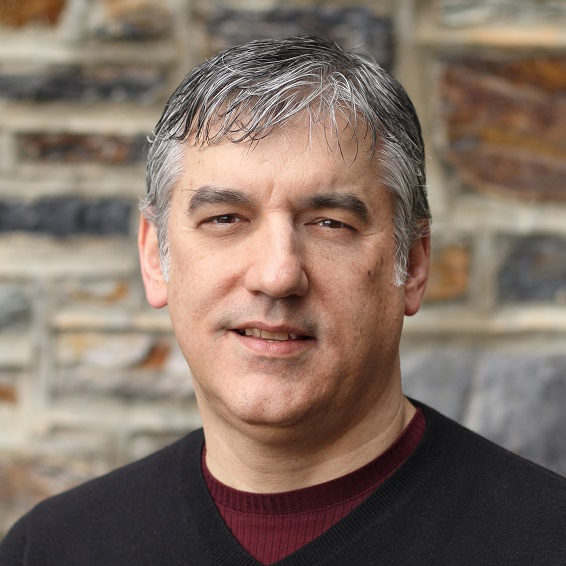
\includegraphics[height=2.1cm]{imgs/members/Chris.jpg}\\Christopher R Monroe};
        \node[align=center,below,font=\tiny] at (0, 0)
        {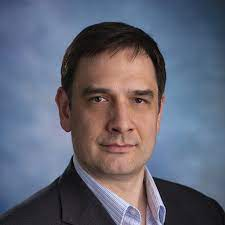
\includegraphics[height=2.1cm]{imgs/members/Alex.jpg}\\Alexander Kozhanov};
        \node[align=center,below,font=\tiny] at (3, 0)
        {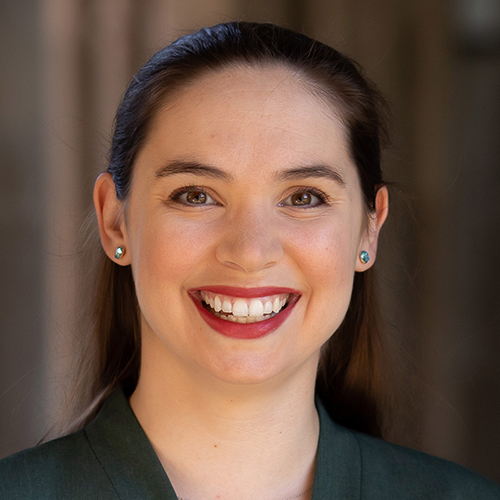
\includegraphics[height=2.1cm]{imgs/members/Crystal.jpg}\\Crystal Noel};

        \shadedraw[inner color=gray,outer color=blue!40!white,path fading = glow2 fading] (-5.8,0.05-3) rectangle (5.8,0.15-3);

        \node[align=center,below,font=\tiny] at (-4.2, -3)
        {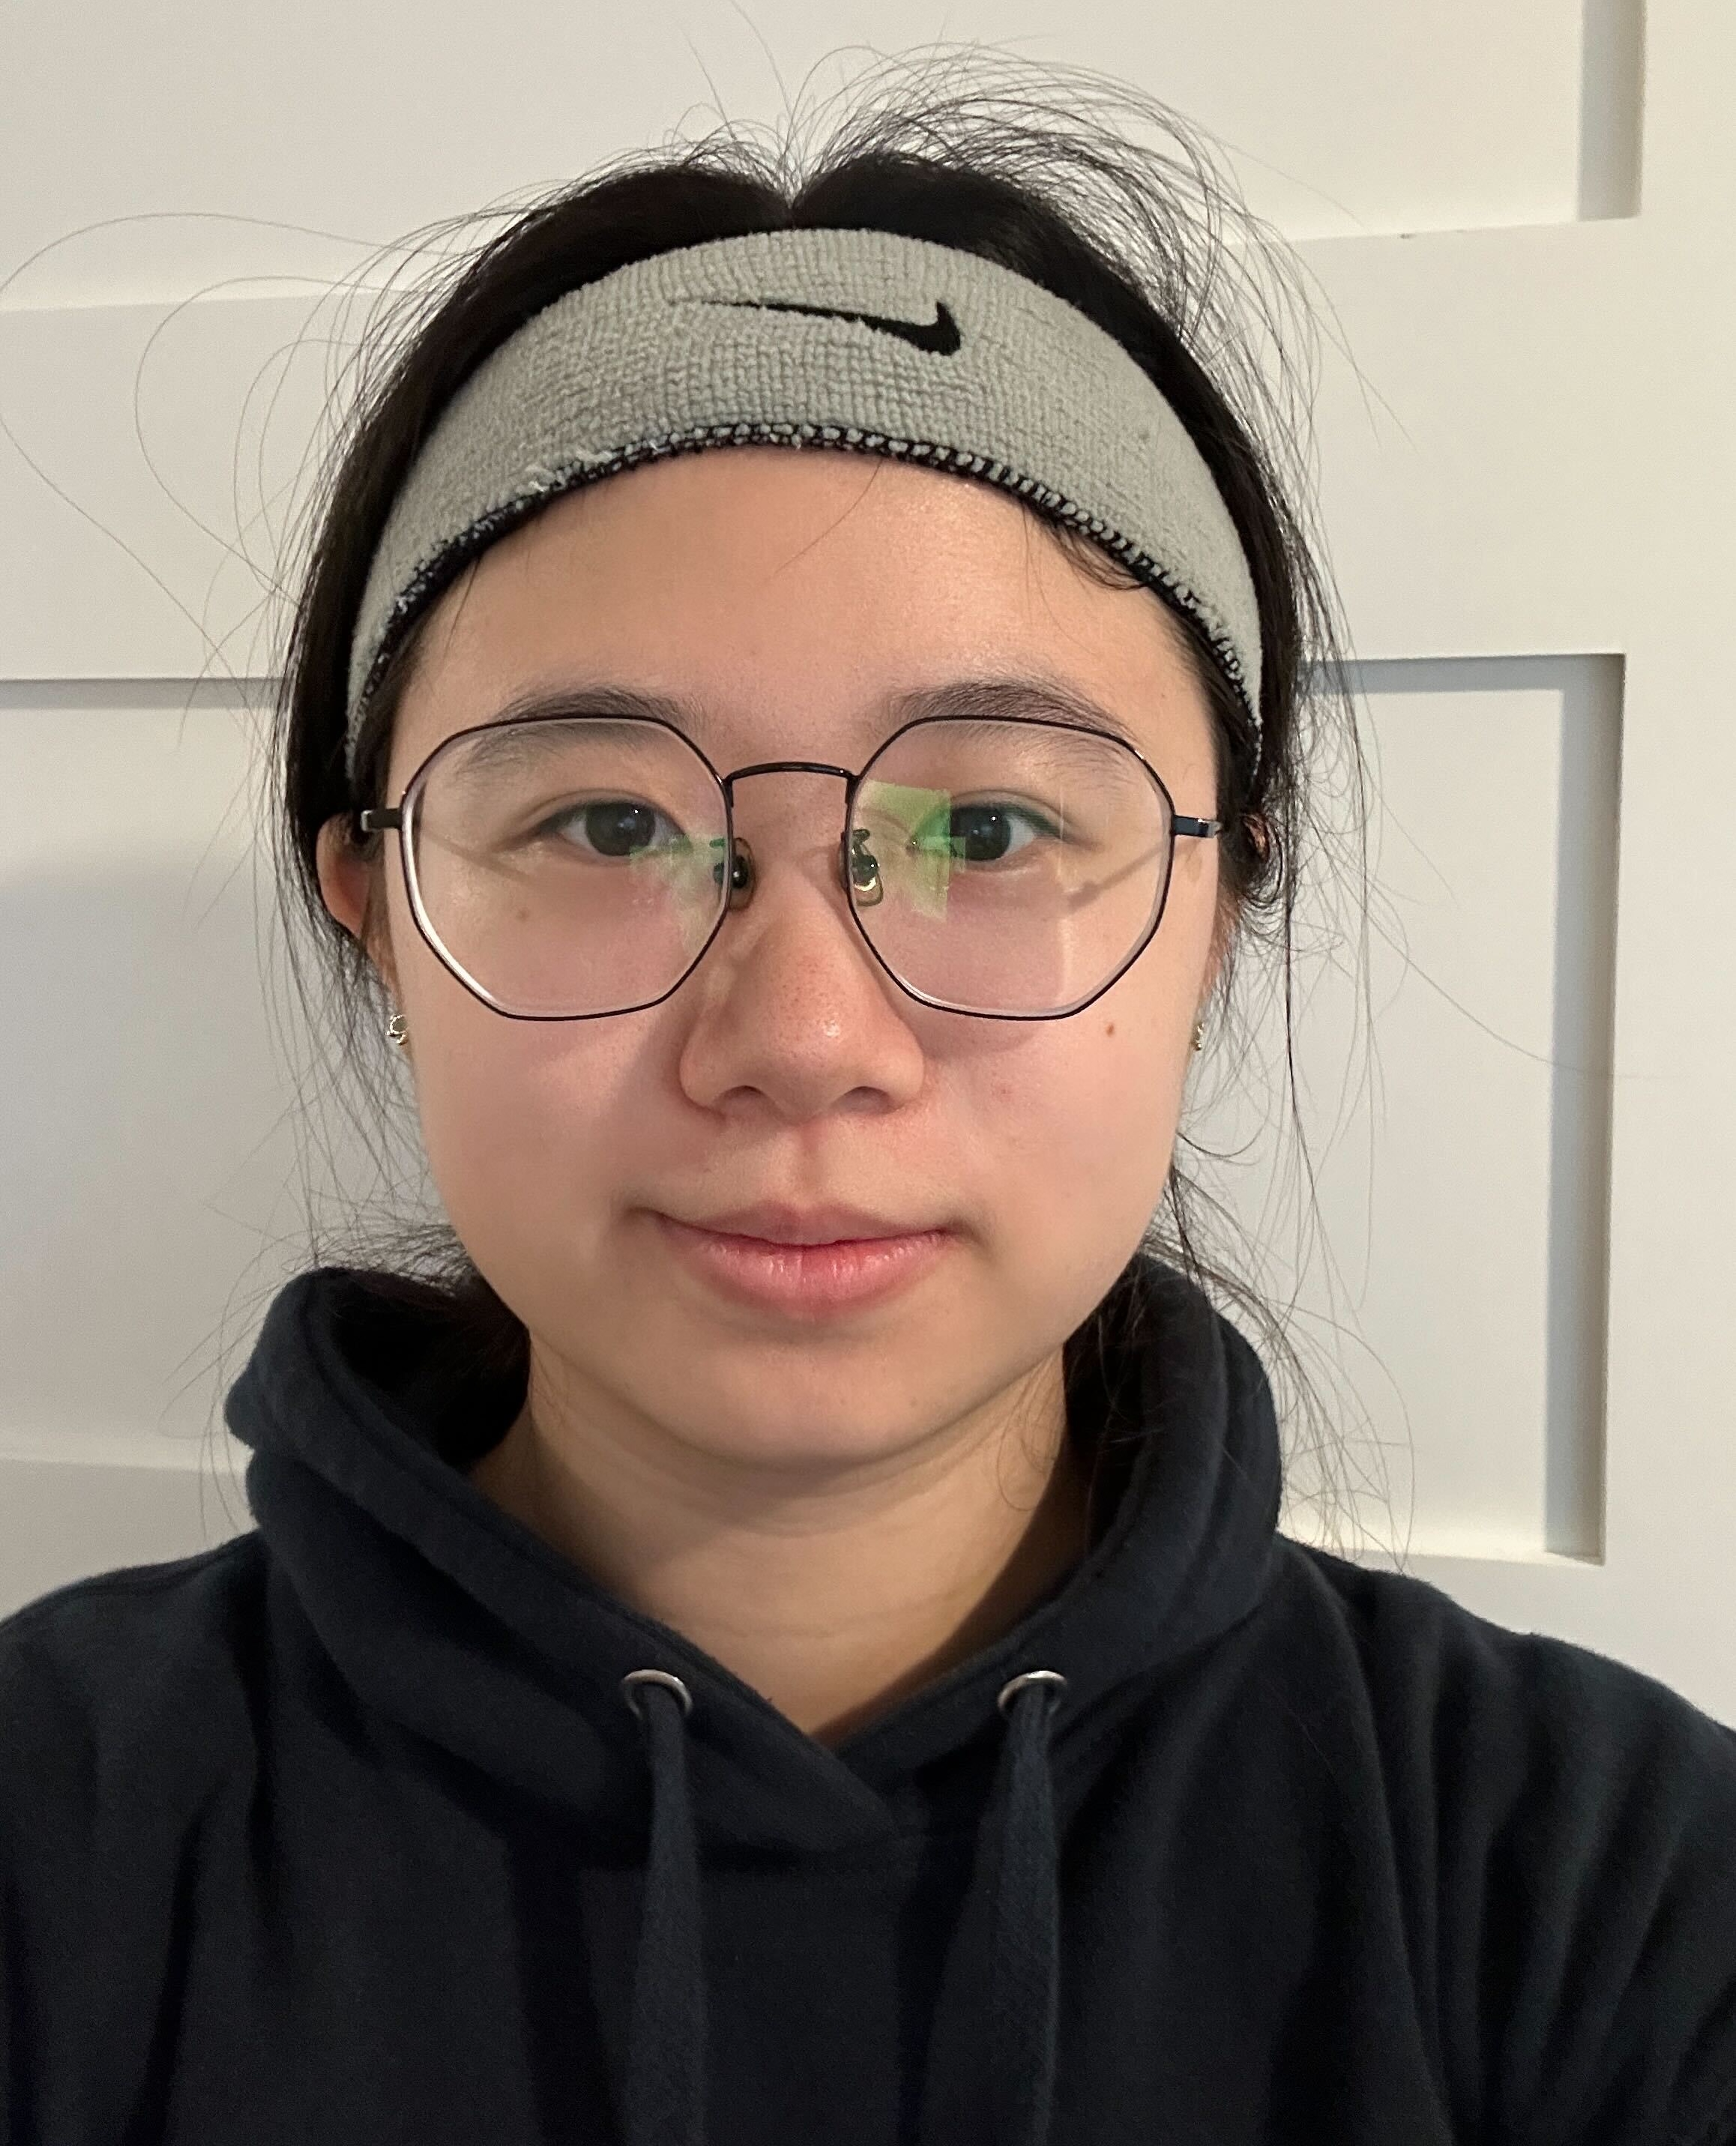
\includegraphics[height=2.1cm]{imgs/members/Keqin.jpg}\\Keqin Yan};
        \node[align=center,below,font=\tiny] at (-1.4, -3)
        {\includegraphics[height=2.1cm]{imgs/members/Vivian.png}\\Vivian Zhang};
        \node[align=center,below,font=\tiny] at (1.4, -3)
        {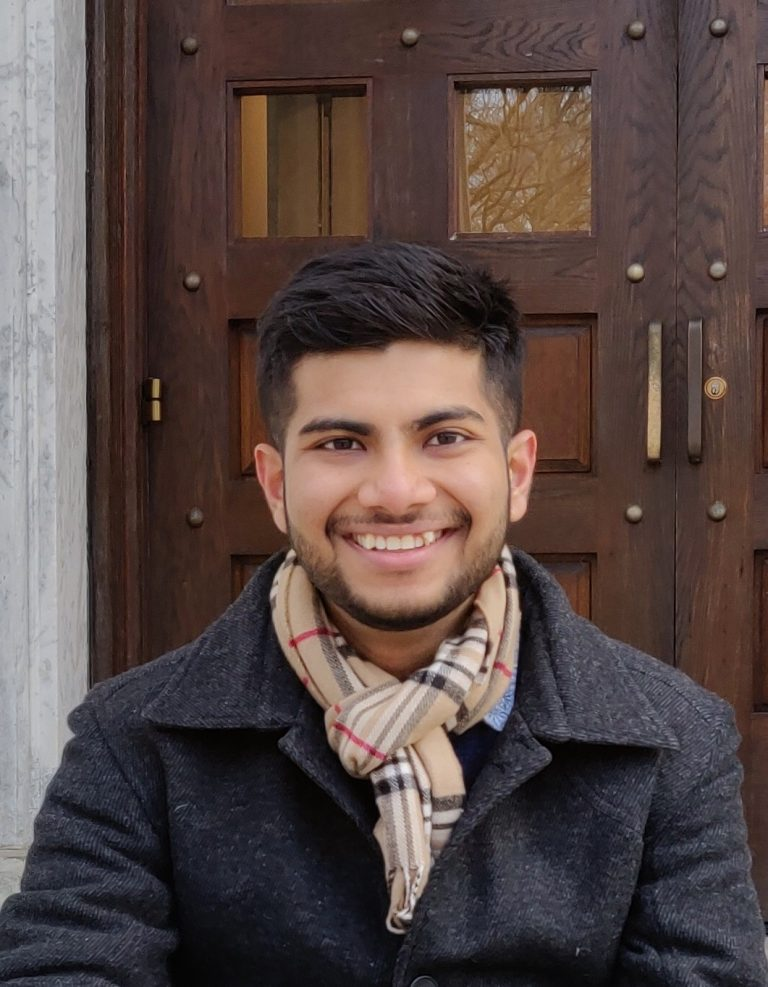
\includegraphics[height=2.1cm]{imgs/members/Debo.jpg}\\Debopriyo Biswas};
        \node[align=center,below,font=\tiny] at (4.2, -3)
        {\includegraphics[height=2.1cm]{imgs/members/Bahaa.jpg}\\Bahaa Harraz};
      \end{tikzpicture}
    \end{center}
  \end{frame}
}

\begin{frame}{}
\end{frame}

\end{document}
